\documentclass[11pt,a4paper]{article}

\usepackage[utf8]{inputenc}
\usepackage[margin=1in]{geometry}
\usepackage{amsmath,amssymb,amsfonts}
\usepackage{graphicx}
\usepackage{booktabs}

\title{\textbf{Predicting Hydrocarbon Fuel Blend Properties from Chemical Composition: A Physics-First Residual Learning Framework with Calibrated Conformal Safety Margins}}

\author{
    \textbf{Kahaan Shah}$^{1,*}$, 
    \textbf{Namyaa Parmar}$^{1}$, 
    \textbf{Arijit Ganguli}$^{1}$,\\
    \textbf{Jayendra Bhalodiya}$^{1}$, 
    \textbf{A. S. K. Sinha}$^{1}$\\[0.5em]
    $^{1}$School of Engineering and Applied Science,\\
    Ahmedabad University, Ahmedabad, Gujarat 380009, India\\[0.3em]
    $^*$Corresponding author: \texttt{kahaan.s2@ahduni.edu.in}
}

\date{\today}

\begin{document}

\maketitle

\begin{abstract}
Rapid pre-screening of novel aviation fuels, sustainable aviation fuel (SAF) blendstocks, and hydrocarbon surrogates demands accurate property prediction directly from chemical composition. However, prevailing data-driven models frequently suffer from two severe methodological flaws: training on synthetic blends generated by empirical formulas (leading to circular, illusory $\sim 0.4\%$ error metrics) and reporting uncalibrated point estimates devoid of statistical safety bounds. In life-critical aviation applications, over-predicting flash point or under-predicting freezing point presents catastrophic operational hazards. 

Here, we present a verified, grey-box modeling framework that pairs classical thermodynamic baselines with symmetric pairwise machine learning residuals and distribution-free, one-sided conformal prediction. Kinematic viscosity is modeled using Refutas blending augmented by a LightGBM pairwise excess function evaluated across chemical descriptors; flash point is predicted via an un-tuned Le Chatelier--Raoult--Antoine formulation; and low-temperature flow is governed by Schroeder--van Laar solid-liquid equilibrium with UNIFAC activity coefficients. Evaluated under strict whole-system holdouts (GroupKFold on InChIKey sets) with pre-declared gates, the pairwise residual cut locked held-out viscosity error from 0.054 to 0.031~ln (a statistically significant bootstrap gain of 0.0233, 95\% CI $[0.0163, 0.0302]$), and flash point achieved an MAE of $2.20^\circ\text{C}$ across 70 real-fuel groups with zero blend parameter fitting. In contrast, deep neural architectures (GNNs, DeepSets) failed pre-declared gates, and real-fuel freezing point showed no skill over a trivial constant ($9.31^\circ\text{C}$ vs. $5.18^\circ\text{C}$ MAE), which we transparently disclose and bound with an infinite margin. 

Applying one-sided conformal risk bounds ($\alpha = 0.10$, guaranteeing 90\% dangerous-side coverage) within a multistart simplex optimizer identified three certified candidate blends out of sixteen tested pools under ASTM D1655 constraints. This study demonstrates that trustworthy computational fuel engineering requires abandoning circular synthetic benchmarks in favor of thermodynamic backbones, rigorous whole-system validation, and distribution-free safety margins.
\end{abstract}

\textbf{Keywords:} Sustainable Aviation Fuels; Hydrocarbon Blending; Machine Learning; Refutas Viscosity; Conformal Prediction; Inverse Molecular Design.

\newpage

\section{Introduction}

The aviation industry faces an urgent dual mandate: reducing lifecycle greenhouse gas emissions through the rapid adoption of Sustainable Aviation Fuels (SAF) while upholding non-negotiable airworthiness and safety standards~\cite{astmd1655, edwards2017reference}. Commercial jet fuels (such as Jet~A and Jet~A-1) are intricate multicomponent mixtures containing hundreds of distinct hydrocarbon isomers spanning paraffins (normal and iso-alkanes), cycloparaffins (naphthenes), and aromatics across the $\text{C}_8$--$\text{C}_{16}$ carbon window. To ensure flight safety, fuels must comply with rigorous physical and transport property thresholds codified in ASTM D1655~\cite{astmd1655}. Among these, four properties are paramount:
\begin{enumerate}
    \item \textbf{Flash Point} ($\ge 38^\circ\text{C}$): Governs flammability during ground handling and storage;
    \item \textbf{Freezing Point} ($\le -40^\circ\text{C}$ for Jet A, $\le -47^\circ\text{C}$ for Jet A-1): Prevents wax crystallization and fuel line filter clogging during prolonged cruise at high altitudes;
    \item \textbf{Kinematic Viscosity} ($\le 8.0\text{ cSt}$ at $-20^\circ\text{C}$): Dictates cold-flow pumpability and fuel spray atomization inside the combustion chamber;
    \item \textbf{Density} ($775\text{ to }840\text{ kg/m}^3$ at $15^\circ\text{C}$): Ensures correct aircraft fuel metering and volumetric energy payload.
\end{enumerate}

Physical laboratory qualification of novel fuel blendstocks via the ASTM D4054 clearing process requires thousands of gallons of experimental fuel and costs millions of dollars~\cite{astmd4054}. Consequently, high-fidelity computational models capable of predicting blend properties directly from molecular composition—and running the process in reverse via \textit{inverse blend design}—are urgently sought.

However, existing literature exhibits two critical vulnerabilities:
\begin{itemize}
    \item \textbf{The Circularity and Data-Leakage Trap:} Numerous recent deep learning studies report deceptively low errors ($\sim 0.4\%$) by training feed-forward networks or graph neural networks (GNNs) on \textit{synthetic} blends generated by classical empirical equations (such as the Refutas formula), or by performing random row-level train/test splits where identical chemical mixtures at slightly varied temperatures or compositions leak across folds~\cite{leenhouts2024benchmarking}. When deployed on real-world fuels, these models degrade precipitously.
    \item \textbf{Absence of Calibrated Safety Bounds:} Standard machine learning architectures emit point estimates. In fuels engineering, error directionality is inherently asymmetric. Over-predicting a flash point ($40^\circ\text{C}$ predicted vs. $36^\circ\text{C}$ actual) erroneously certifies a dangerous fuel as safe; under-predicting a freezing point ($-45^\circ\text{C}$ predicted vs. $-38^\circ\text{C}$ actual) risks catastrophic in-flight fuel system freezing.
\end{itemize}

To overcome these barriers, this study establishes a \textit{physics-first, grey-box} methodology governed by strict pre-declared evaluation contracts, locked whole-system holdouts, and distribution-free conformal prediction~\cite{vovk2005algorithmic, angelopoulos2023conformal}. Rather than attempting to replace thermodynamics with unconstrained black-box models, we leverage verified physical baselines (Refutas, ideal Le Chatelier, and Schroeder--van Laar) and employ machine learning strictly to learn residual pairwise non-idealities where empirical evidence demonstrates provable skill.

\section{Theoretical Foundations}

\subsection{Composition Representations}
Let a multicomponent fuel blend contain $N$ distinct hydrocarbon components, each defined by mass fraction $w_i$, molar mass $M_i$, and temperature-dependent liquid density $\rho_i(T)$. Because different thermodynamic phenomena depend on distinct molecular bases, fractions are converted as:
\begin{equation}
    x_i = \frac{w_i / M_i}{\sum_{j=1}^N (w_j / M_j)}, \quad v_i = \frac{w_i / \rho_i(T)}{\sum_{j=1}^N (w_j / \rho_j(T))}
\end{equation}
where $x_i$ denotes liquid mole fraction (governing vapor-liquid and solid-liquid equilibria) and $v_i$ denotes liquid volume fraction (governing volumetric and empirical blending).

\subsection{Classical Thermodynamic Baselines}

\subsubsection{Density: Ideal Volume Mixing}
Hydrocarbon mixtures exhibit minimal excess molar volume of mixing ($< 0.5\%$). Liquid blend density $\rho_{\text{mix}}$ is computed under ideal volume additivity:
\begin{equation}
    \frac{1}{\rho_{\text{mix}}(T)} = \sum_{i=1}^N \frac{w_i}{\rho_i(T)}
    \label{eq:dens_ideal}
\end{equation}

\subsubsection{Kinematic Viscosity: The Refutas Blending Index}
Viscosity exhibits extreme non-linearity upon mixing. The empirical petroleum standard, Refutas~\cite{maples2000petroleum}, maps each component's kinematic viscosity $\nu_i$ (in cSt, $\text{mm}^2/\text{s}$) to a Viscosity Blending Number ($\text{VBN}_i$):
\begin{equation}
    \text{VBN}_i = 14.534 \cdot \ln\left(\ln(\nu_i + 0.8)\right) + 10.975
\end{equation}
VBN combines linearly on a mass basis:
\begin{equation}
    \text{VBN}_{\text{mix}} = \sum_{i=1}^N w_i \cdot \text{VBN}_i
\end{equation}
from which the blend viscosity is recovered:
\begin{equation}
    \nu_{\text{mix}} = \exp\left(\exp\left(\frac{\text{VBN}_{\text{mix}} - 10.975}{14.534}\right)\right) - 0.8
    \label{eq:refutas}
\end{equation}

\subsubsection{Flash Point: Le Chatelier--Raoult--Antoine Flammability}
Flash point is the lowest liquid temperature at which the equilibrium headspace vapor attains the lower flammability limit (LFL)~\cite{lechatelier1891estimation}. Pure-component saturation pressures $P_i^{\text{sat}}(T)$ are computed via the Antoine equation:
\begin{equation}
    \log_{10} P_i^{\text{sat}}(T) = A_i - \frac{B_i}{T + C_i} \quad [P \text{ in kPa}, T \text{ in K}]
\end{equation}
Historically, standard Antoine constants compiled in databases such as the NIST Chemistry WebBook were regressed from boiling-point measurements at elevated temperatures ($95\text{ to }190^\circ\text{C}$). When extrapolated downward into the sub-ambient to ambient flash point window ($0\text{ to }60^\circ\text{C}$), these parameters severely underestimate vapor pressure, leading to severe negative flash point prediction errors (historically as severe as $-21.7^\circ\text{C}$). In this work, Antoine constants for all key kerosene hydrocarbons are re-anchored and refitted against experimental vapor pressure measurements specifically in the $0\text{ to }100^\circ\text{C}$ window, eliminating this systematic bias.

Assuming ideal vapor-liquid equilibrium (Raoult's law, total pressure $P_{\text{tot}} = 101.325\text{ kPa}$), the equilibrium vapor mole fraction is $y_i(T) = x_i P_i^{\text{sat}}(T) / P_{\text{tot}}$. The flammability hazard index $H(T)$ combines species contributions via Le Chatelier's rule:
\begin{equation}
    H(T) = \sum_{i=1}^N \frac{y_i(T)}{\text{LFL}_i(T)} = \sum_{i=1}^N \frac{x_i P_i^{\text{sat}}(T)}{P_{\text{tot}} \cdot \text{LFL}_i(T)}
    \label{eq:le_chatelier}
\end{equation}
where $\text{LFL}_i(T)$ is corrected for temperature via Zabetakis' relation~\cite{zabetakis1965flammability}:
\begin{equation}
    \text{LFL}_i(T) = \text{LFL}_{i, 25^\circ\text{C}} \left[ 1 - 0.000721 \cdot (T - 298.15) \right]
\end{equation}
The flash point $T_{\text{flash}}$ is the exact root satisfying $H(T) - 1 = 0$, solved numerically using Brent's method on $[150\text{ K}, 650\text{ K}]$. Crucially, this model requires zero parameters fitted to mixture flash data.

\subsubsection{Freezing Point: Schroeder--van Laar Solid-Liquid Equilibrium}
Crystallization onset of component $i$ from a liquid mixture is modeled via the Schroeder--van Laar equation~\cite{schroeder1893erstarrung}:
\begin{equation}
    \frac{1}{T_i} = \frac{1}{T_{m,i}} - \frac{R \ln(x_i \gamma_i)}{\Delta H_{\text{fus},i}}
    \label{eq:svl}
\end{equation}
where $T_{m,i}$ is melting temperature, $\Delta H_{\text{fus},i}$ is enthalpy of fusion, $R$ is the universal gas constant, and $\gamma_i$ is the liquid-phase activity coefficient estimated via the original UNIFAC group-contribution method~\cite{fredenslund1975group}. The mixture crystallization onset occurs at $T_{\text{freeze}} = \max_{1 \le i \le N} T_i$.

\section{Methodology}

\subsection{Data Curation and Refusal Policy}
To eliminate data contamination, we assembled experimental measurements from five primary sources:
\begin{enumerate}
    \item \textbf{Leenhouts Benchmark Dataset}~\cite{leenhouts2024benchmarking}: Curated pure and mixture flash points, viscosities, and ignition qualities;
    \item \textbf{NIST/TDE Viscosity Database}: Binary viscosity measurements reconciled from raw Pa$\cdot$s units;
    \item \textbf{NIST ThermoML Archive}: Measured liquid densities, viscosities, and vapor pressures (re-extracted to resolve historical phase and constraint parsing anomalies);
    \item \textbf{Coordinating Research Council (CRC) Report 647}~\cite{crc647report}: Property tables for 57 real aviation fuels with compositions reconstructed from measured hydrocarbon class distributions (Table G.1);
    \item \textbf{Alternative Jet Fuels Test Database (AJFTD)}: Comprehensive property tables for real petroleum and synthetic fuels, including 116 fuels characterized via comprehensive two-dimensional gas chromatography ($\text{GC}\times\text{GC}$).
\end{enumerate}

\textbf{Explicit Data Refusal:} We explicitly quarantined and banned synthetic mixture datasets (such as \texttt{DatasetsFuelProperties.xlsx}, containing 50,000 synthetic rows generated from the Refutas equation) and legacy formula-derived fuel corpuses. Exact experimental duplicates were collapsed to their median; all measurement units were standardized to SI/canonical units.

\subsection{Pairwise Residual Machine Learning}
While Refutas captures bulk viscosity trends, it ignores specific intermolecular pair interactions. Drawing inspiration from the Grunberg--Nissan framework~\cite{grunberg1949mixture}, we decompose the mixture viscosity into the physical baseline plus an excess pairwise correction:
\begin{equation}
    \ln \eta_{\text{mix}} = \ln \eta_{\text{Refutas}} + \sum_{i < j} x_i x_j \cdot g(d_i, d_j, T)
    \label{eq:visc_pair}
\end{equation}
where $g(d_i, d_j, T)$ is a symmetric scalar function evaluated on the molecular descriptor vector $d_i, d_j$ of the interacting pair. 

The correction $g$ is learned via LightGBM~\cite{ke2017lightgbm} (400 trees, 15 leaves, learning rate 0.05, deterministic seed 42). The input feature vector consists of:
\begin{equation}
    \Phi_{ij}(T) = \left[ \bar{C}_{ij}, |\Delta C_{ij}|, \bar{M}_{ij}, |\Delta M_{ij}|, \bar{R}_{ij}, |\Delta R_{ij}|, \overline{\text{CH}}_3, \bar{Q}_C, \overline{\ln \eta_i}, \bar{V}_{m}, \text{ClassPair}_{ij}, \frac{1}{T} \right]
\end{equation}
where $\bar{C}$ and $|\Delta C|$ represent the mean and absolute difference in carbon number, $M$ is molar mass, $R$ is ring count, $Q_C$ is quaternary carbon count, and $V_m$ is molar volume. This pairwise formulation guarantees:
\begin{enumerate}
    \item \textbf{Permutation Invariance:} Summation over $i < j$ is naturally symmetric under component reordering;
    \item \textbf{Pure-Component Recovery:} As $x_i \to 1$, all cross-products $x_i x_j \to 0$, exactly preserving pure-component physics;
    \item \textbf{Arbitrary Composition Scalability:} A model trained strictly on binary pairs extends directly to $N$-component blends without architectural alteration.
\end{enumerate}

\subsection{Uncertainty Quantification via One-Sided Conformal Prediction}
For safety-critical engineering, point predictions must be augmented with statistical coverage guarantees. We employ distribution-free split conformal inference~\cite{vovk2005algorithmic, angelopoulos2023conformal}.

Let $g \in \{1, \dots, n\}$ index independent held-out chemical systems. For a given property, the dangerous-side non-conformity score $s_g$ is defined as the worst-case error on system $g$:
\begin{equation}
    s_g = \max_{p \in g} \left( \hat{y}_p - y_p \right) \quad [\text{for properties where over-prediction is dangerous, e.g., flash point}]
\end{equation}
\begin{equation}
    s_g = \max_{p \in g} \left( y_p - \hat{y}_p \right) \quad [\text{for properties where under-prediction is dangerous, e.g., freezing point}]
\end{equation}
Given $n$ calibration systems and a target error rate $\alpha = 0.10$ (90\% one-sided confidence), the conformal rank index is:
\begin{equation}
    k = \left\lceil (n + 1)(1 - \alpha) \right\rceil
\end{equation}
The conformal safety margin is the $k$-th order statistic: $\text{Margin}_{90} = s_{(k)}$. If $k > n$, the data cannot support a 90\% guarantee without distributional extrapolation, and the margin is rigorously set to $\infty$.

\textbf{Definition of ``Certified'':} A candidate blend is defined as \textit{model-certified} if and only if:
\begin{enumerate}
    \item A finite conformal margin exists for all constrained properties;
    \item All components reside within the defined model applicability domain;
    \item The predicted value satisfies the specification limit \textit{after} the one-sided margin is applied:
    \begin{align}
        \hat{T}_{\text{flash}} - \text{Margin}_{\text{flash}} &\ge 38.0^\circ\text{C} \\
        \hat{T}_{\text{freeze}} + \text{Margin}_{\text{freeze}} &\le -40.0^\circ\text{C} \quad (\text{Jet A}) \\
        \hat{\nu}_{-20^\circ\text{C}} \cdot \exp(\text{Margin}_{\ln \nu}) &\le 8.0\text{ cSt}
    \end{align}
\end{enumerate}

\subsection{Evaluation Contract: Whole-System Holdout and Trivial Baselines}
All models were governed by pre-declared gates committed to the repository before scoring:
\begin{itemize}
    \item \textbf{System-Level GroupKFold:} Cross-validation folds were partitioned strictly by \texttt{system\_id} (the MD5 hash of sorted component InChIKeys). No two measurements sharing the same molecular system were ever split across train and test.
    \item \textbf{Trivial Comparator:} Every model was benchmarked against a leave-one-group-out constant predictor ($\bar{y}_{-g}$). Models failing to outperform this trivial baseline received a verdict of \texttt{no\_skill\_shown} and were barred from claiming predictive skill.
\end{itemize}

\subsection{Inverse Blend Optimization}
The inverse design problem seeks a component mass fraction vector $\mathbf{w} \in \mathbb{R}^N$ lying on the unit simplex:
\begin{equation}
    \Delta^{N-1} = \left\{ \mathbf{w} \in \mathbb{R}^N : \sum_{i=1}^N w_i = 1, \; w_i \ge 0 \right\}
\end{equation}
Optimization is conducted via multistart Sequential Least Squares Programming (SLSQP, 10 restarts, seed 42) maximizing the minimum margin-adjusted slack across all active ASTM D1655 constraints:
\begin{equation}
    \max_{\mathbf{w} \in \Delta^{N-1}} \; \min_{m \in \mathcal{M}} \left[ \text{Slack}_m(\mathbf{w}) \right]
\end{equation}
where $\text{Slack}_m(\mathbf{w}) = \text{Limit}_m - \left( \hat{y}_m(\mathbf{w}) \pm \text{Margin}_m \right)$. Distillation boiling curves ($T_{10}, T_{50}, T_{90}$) are evaluated using the empirical Engler D86 correlation; an alternative Rayleigh distillation model was evaluated during development but rejected because its $+11.6^\circ\text{C}$ bias on $T_{10}$ failed pre-declared adoption gates. 

Crucially, the optimizer enforces a strict fail-safe constraint protocol: if an optimization constraint specifies a property whose conformal margin is infinite (such as real-fuel viscosity below $263\text{ K}$, where no proven skill over a constant exists), the optimization engine strictly refuses to drop or relax the constraint. Instead, it immediately halts execution and raises a \texttt{ModelUnavailable} exception, guaranteeing that uncertifiable blends cannot be falsely emitted.

\newpage

\section{Results}

\subsection{Kinematic Viscosity: Pre-Declared Gate Verification}
The pairwise LightGBM residual model was trained on 264 binary systems and scored against four pre-declared gates. As documented in Table~\ref{tab:visc_gates}, the model passed all four gates with statistically validated gains.

\begin{table}[htbp]
\centering
\caption{Pre-declared evaluation gate results for kinematic viscosity pairwise residual ($\ln \eta$). Gain confidence intervals (95\%) are derived via system-level group bootstrap.}
\label{tab:visc_gates}
\resizebox{\textwidth}{!}{
\begin{tabular}{llcccccc}
\toprule
\textbf{Gate} & \textbf{Evaluation Set} & \textbf{$N_{\text{sys}}$} & \textbf{MAE (Refutas)} & \textbf{MAE (Pair ML)} & \textbf{Gain} & \textbf{95\% CI} & \textbf{Outcome} \\
\midrule
R-MLV-1 & Dev (System OOF) & 264 & 0.0824 & 0.0599 & 0.0225 & $[0.0180, 0.0269]$ & \textbf{PASS} \\
R-MLV-2 & Locked Holdout & 70 & 0.0544 & 0.0311 & 0.0233 & $[0.0163, 0.0302]$ & \textbf{PASS} \\
R-MLV-3 & Ternaries+ (System Macro) & 18 & 0.0985 & 0.0419 & 0.0565 & $[0.0401, 0.0737]$ & \textbf{PASS} \\
R-MLV-4 & Cold Mixtures ($< 283\text{ K}$) & 26 & 0.0994 & 0.0612 & 0.0382 & $[0.0225, 0.0547]$ & \textbf{PASS} \\
\bottomrule
\end{tabular}
}
\end{table}

On the 70 locked held-out systems, the pairwise model reduced Refutas error by 43\%, dropping MAE from 0.0544 to 0.0311~ln. The bootstrap confidence interval of the gain ($[0.0163, 0.0302]$) strictly excludes zero, decisively outperforming a constant-offset comparator (MAE 0.0431). Figure~\ref{fig:visc_parity} illustrates the parity comparison between Refutas and the pairwise ML residual on held-out systems.

\begin{figure}[htbp]
    \centering
    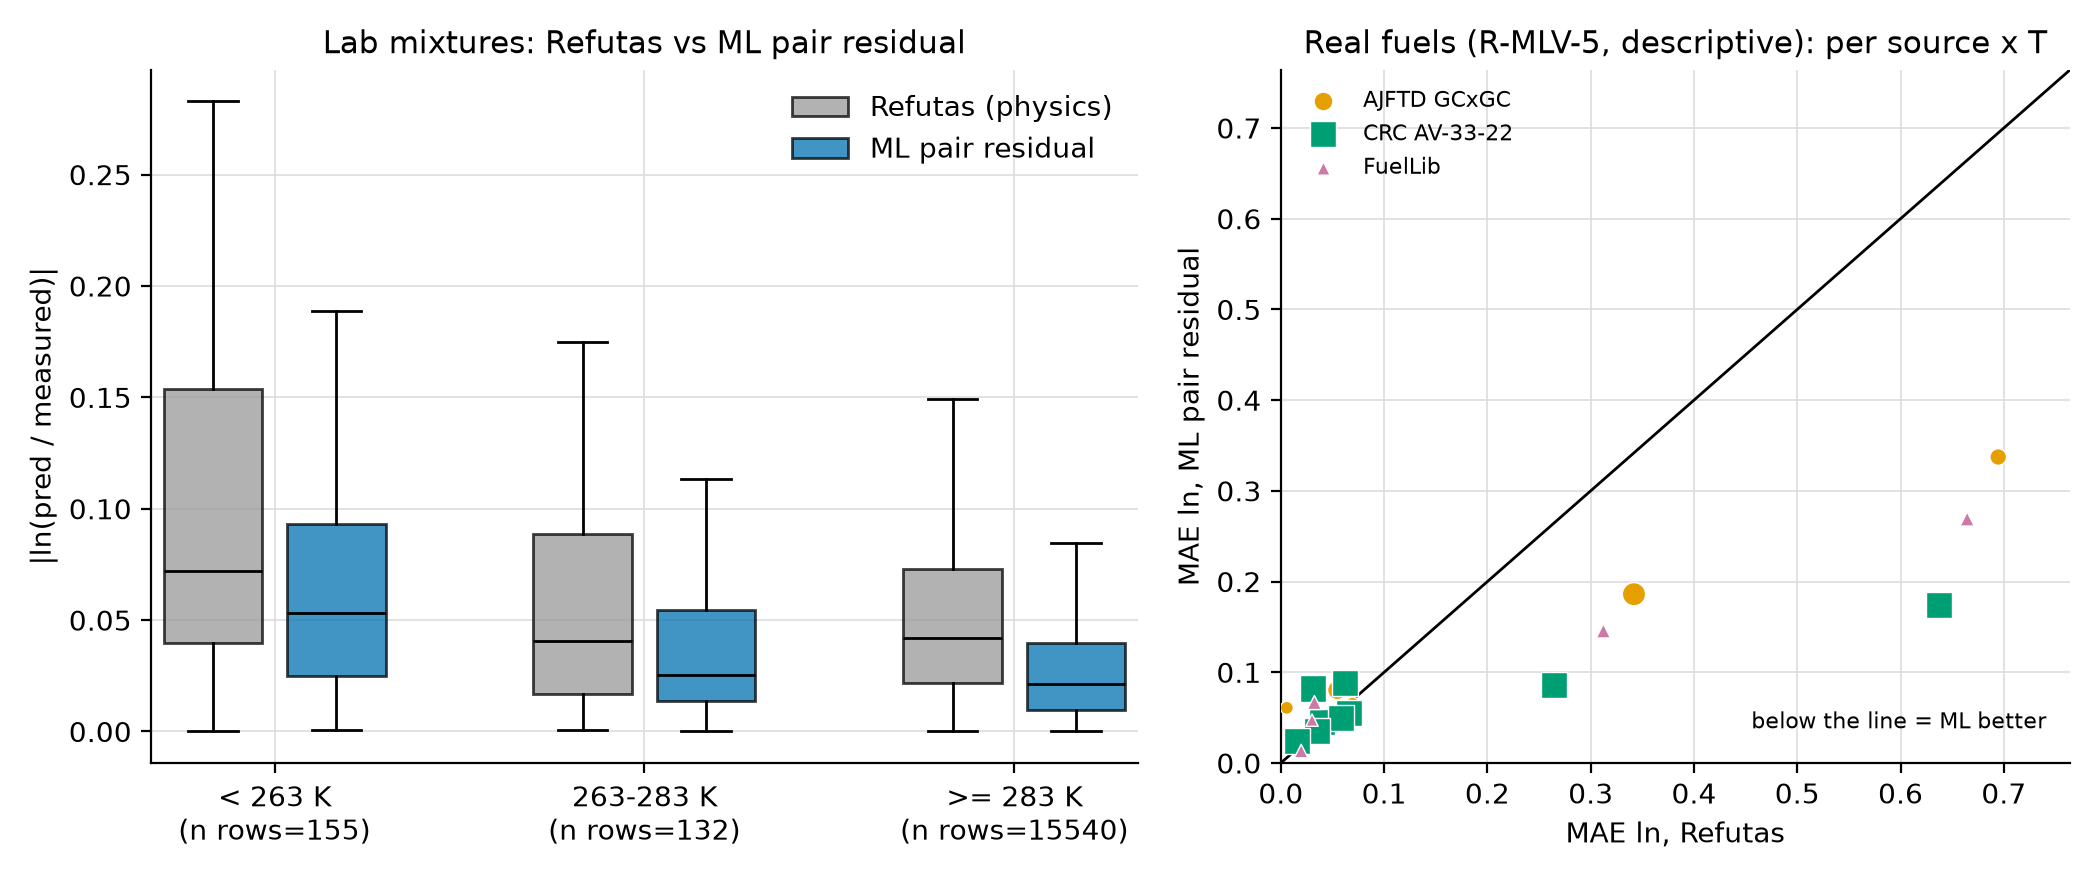
\includegraphics[width=0.75\textwidth]{figures/b_viscosity_refutas_vs_ml.png}
    \caption{Parity comparison of kinematic viscosity predictions on held-out test systems: baseline Refutas (left) vs. pairwise LightGBM residual model (right).}
    \label{fig:visc_parity}
\end{figure}

\subsection{Flash Point Benchmark across Real-Fuel Cohorts}
The un-tuned Le Chatelier--Raoult--Antoine model was evaluated across 70 real-fuel groups from the AJFTD and CRC databases. As detailed in Table~\ref{tab:headline}, the physical model achieved an MAE of $2.196^\circ\text{C}$ with an exceptionally low bias of $+0.059^\circ\text{C}$, vastly outperforming the leave-one-group-out trivial comparator ($5.156^\circ\text{C}$). Across 31 $\text{GC}\times\text{GC}$ characterized fuels, the bias was $-0.152^\circ\text{C}$ with an MAE of $2.995^\circ\text{C}$ (\texttt{beats\_trivial}).

\begin{table}[htbp]
\centering
\caption{Headline property performance on real fuels and locked benchmarks against trivial comparators.}
\label{tab:headline}
\resizebox{\textwidth}{!}{
\begin{tabular}{llccccc}
\toprule
\textbf{Property} & \textbf{Dataset} & \textbf{$N_{\text{groups}}$} & \textbf{Bias} & \textbf{MAE} & \textbf{MAE$_{\text{triv}}$} & \textbf{Verdict} \\
\midrule
Flash Point ($^\circ\text{C}$) & Real Fuels (Pooled) & 70 & $+0.059$ & 2.196 & 5.156 & \texttt{beats\_trivial} \\
Flash Point ($^\circ\text{C}$) & AJFTD $\text{GC}\times\text{GC}$ & 31 & $-0.152$ & 2.995 & 3.977 & \texttt{beats\_trivial} \\
Density ($\text{kg/m}^3$) & Real Fuels ($T \ge 283\text{ K}$) & 69 & $-2.378$ & 4.153 & 16.480 & \texttt{beats\_trivial} \\
Density ($\text{kg/m}^3$) & Lab Mixtures & 167 & $+0.258$ & 1.353 & --- & \texttt{in\_domain} \\
Freezing Point ($^\circ\text{C}$) & Lab Liquidus ($S_F$) & 12 & $+2.466$ & 3.935 & 15.630 & \texttt{beats\_trivial} \\
Freezing Point ($^\circ\text{C}$) & Real Fuels (Pooled) & 50 & $+5.878$ & 8.425 & 6.413 & \textbf{\texttt{no\_skill\_shown}} \\
Freezing Point ($^\circ\text{C}$) & Real Fuels (Locked) & 8 & $+4.286$ & 9.310 & 5.176 & \textbf{\texttt{worse\_than\_trivial}} \\
Cold Viscosity ($< 263\text{ K}$) & Real Fuels (Refutas) & 65 & $-0.505$ & 0.527 & 0.253 & \textbf{\texttt{worse\_than\_trivial}} \\
\bottomrule
\end{tabular}
}
\end{table}

The one-sided conformal safety margin derived across 35 independent laboratory systems is \textbf{$+2.207^\circ\text{C}$}. Parity and distribution curves are shown in Figure~\ref{fig:flash_parity}.

\begin{figure}[htbp]
    \centering
    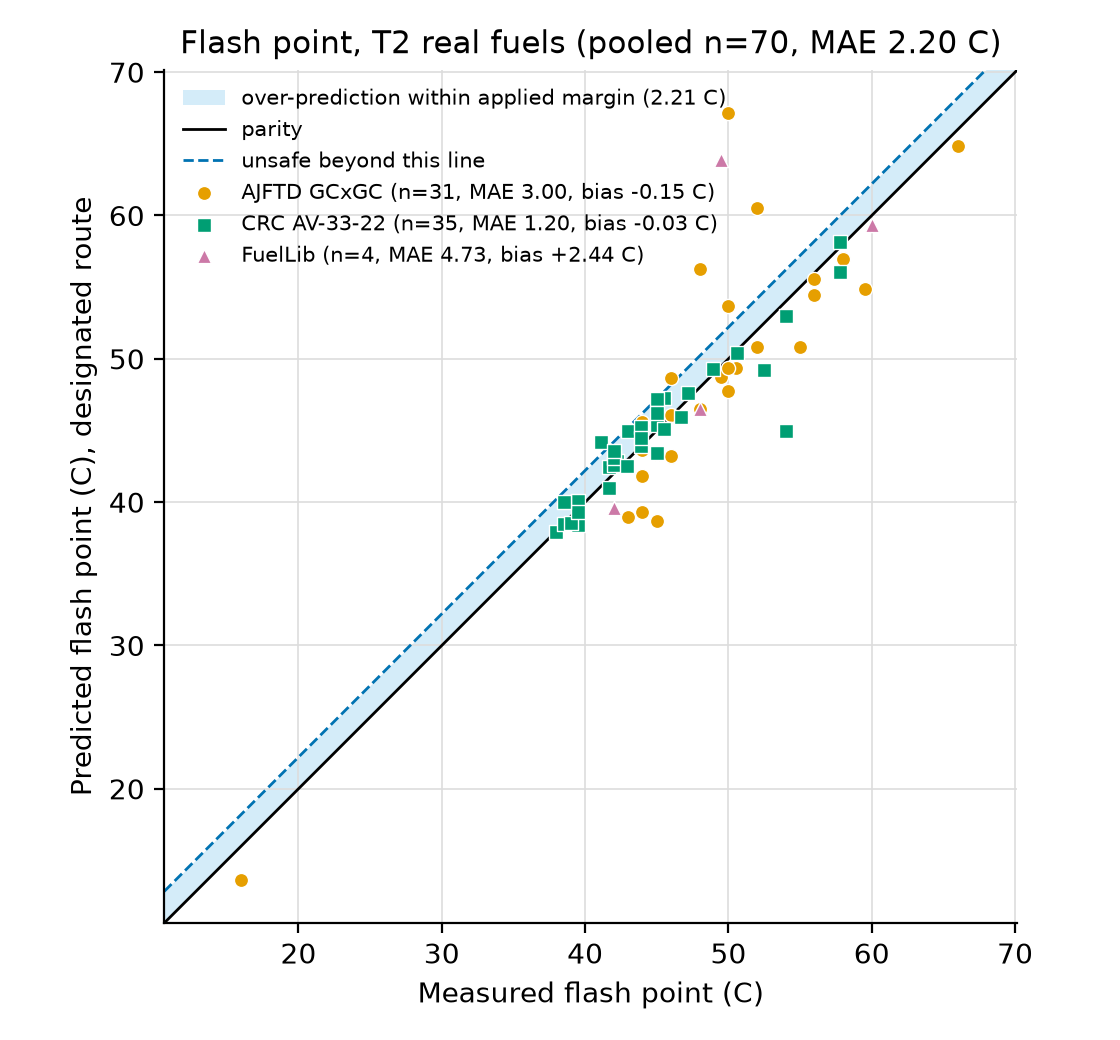
\includegraphics[width=0.75\textwidth]{figures/a_flash_parity_t2.png}
    \caption{Flash point prediction parity on real-fuel test cohorts using the un-tuned anchored Le Chatelier--Raoult formulation.}
    \label{fig:flash_parity}
\end{figure}

\subsection{Honest Negative Results and the Limits of Mixture ML}
A core commitment of this work is the permanent preservation of negative results. Several hypotheses failed their pre-declared gates:
\begin{enumerate}
    \item \textbf{Failure of Complex Neural Mixture Encoders:} Permutation-invariant DeepSets and Graph Neural Networks (GNNs) failed to beat the pairwise LightGBM model on held-out viscosity systems (GNN MAE degraded to 0.040 ln vs. 0.031 ln for LightGBM).
    \item \textbf{Failure of Graph-Estimated Activity Coefficients:} A Graph-Hamiltonian neural network (GH-GNN) trained to predict non-ideal activity coefficients in flash point degraded accuracy by $+0.70^\circ\text{C}$ on lab mixtures and $+1.09^\circ\text{C}$ on real fuels compared to ideal Raoult's law.
    \item \textbf{The Real-Fuel Freezing Point Breakdown:} While UNIFAC-SvL showed skill on 12 laboratory alkane mixtures (MAE $3.935^\circ\text{C}$, margin $13.84^\circ\text{C}$), it performed worse than a constant guess on real fuels (MAE $9.310^\circ\text{C}$ vs. $5.176^\circ\text{C}$, Table~\ref{tab:headline}). Real fuels contain trace heavy paraffins whose non-equilibrium crystallization kinetics cannot be captured by thermodynamic equilibrium group-contribution models.
    \item \textbf{Cold-Temperature Viscosity Breakdown:} Below $263\text{ K}$, Refutas under-predicts real-fuel viscosity significantly (MAE $0.527$ vs. $0.253$ ln for trivial baseline), forcing the real-fuel cold viscosity margin to $\infty$.
\end{enumerate}

\subsection{Conformal Safety Margins and Specification Compliance}
Table~\ref{tab:margins} summarizes the applied one-sided conformal safety margins against ASTM D1655 specification limits. Figure~\ref{fig:margins_spec} demonstrates how the conformal bounds enforce safety headroom during evaluation.

\begin{table}[htbp]
\centering
\caption{Calibrated one-sided conformal safety margins ($\alpha = 0.10$, 90\% coverage) and target ASTM D1655 limits.}
\label{tab:margins}
\resizebox{\textwidth}{!}{
\begin{tabular}{llcccc}
\toprule
\textbf{Property} & \textbf{Governing Model} & \textbf{Dangerous Side} & \textbf{Applied Margin} & \textbf{Calibration Basis} & \textbf{ASTM D1655 Limit} \\
\midrule
Flash Point & Anchored Le Chatelier & Over-prediction & $+2.207^\circ\text{C}$ & 35 lab systems & $\ge 38.0^\circ\text{C}$ \\
Freezing Point & UNIFAC-SvL & Under-prediction & $+13.843^\circ\text{C}$ & 12 lab systems & $\le -40.0^\circ\text{C}$ (Jet A) \\
Density ($15^\circ\text{C}$) & Ideal Volume & Two-sided & $+4.587 / -3.250\text{ kg/m}^3$ & 167 systems & $775\text{ to }840\text{ kg/m}^3$ \\
Viscosity ($\ge 283\text{ K}$) & Pairwise LightGBM & Two-sided & $\pm 0.1343\text{ ln}$ & 264 systems & --- \\
Viscosity ($< 263\text{ K}$) & Refutas (Real Fuels) & Two-sided & $\infty$ & Insufficient skill & $\le 8.0\text{ cSt at } -20^\circ\text{C}$ \\
\bottomrule
\end{tabular}
}
\end{table}

\begin{figure}[htbp]
    \centering
    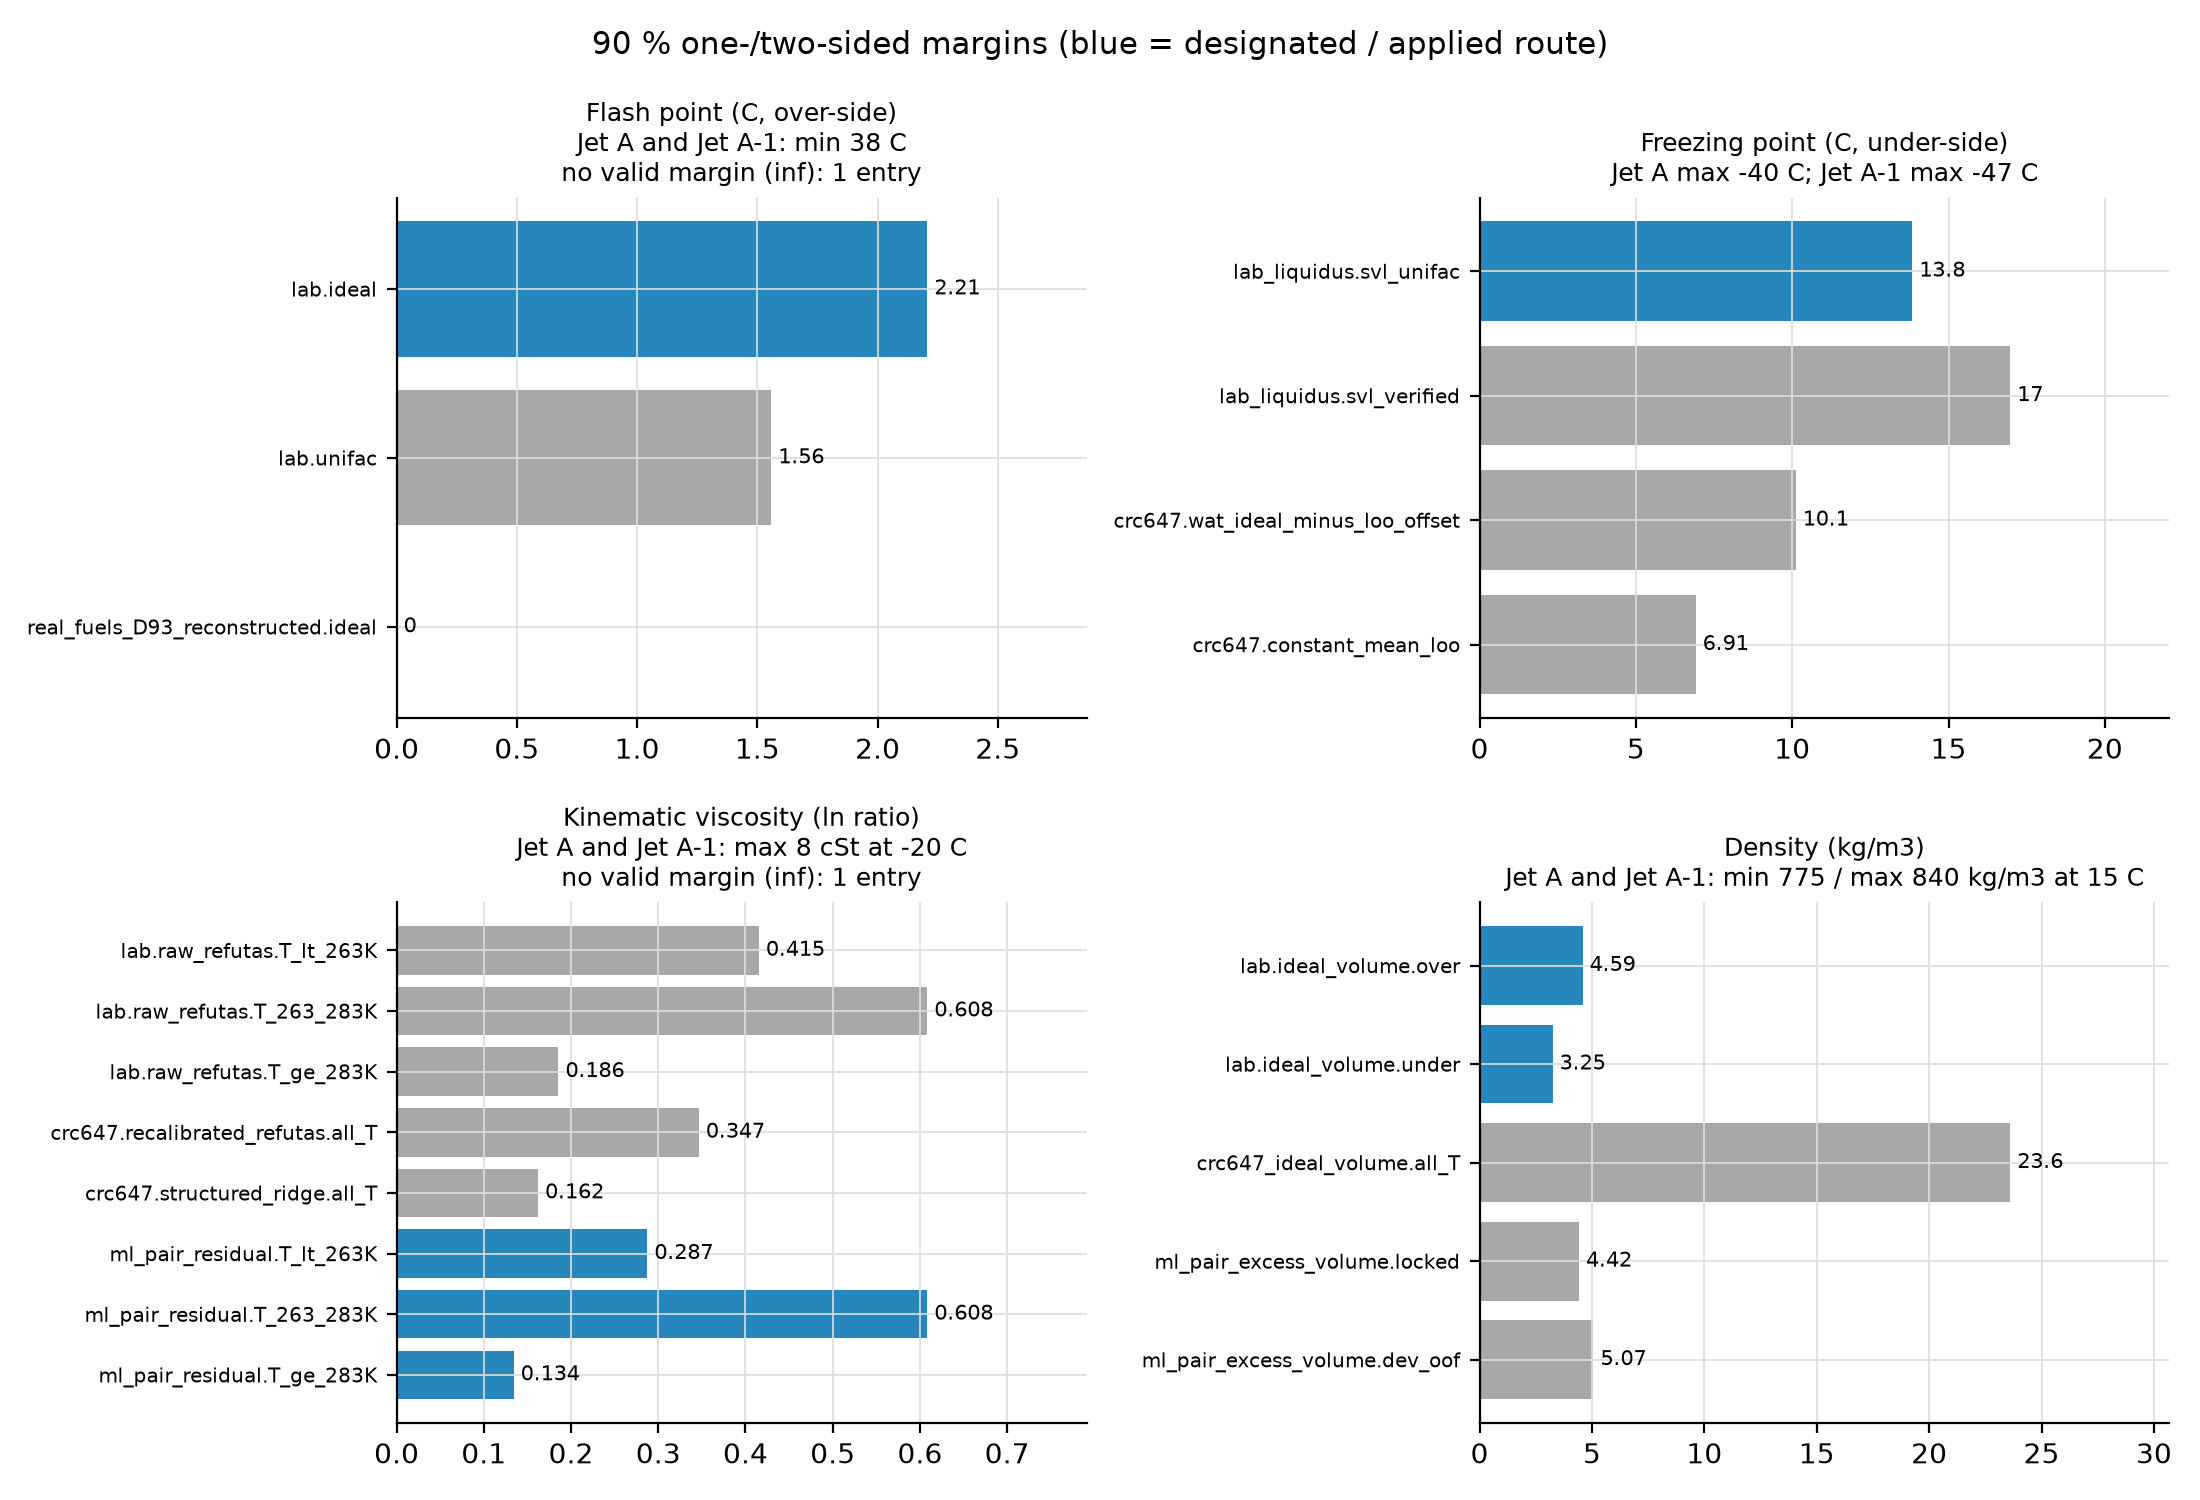
\includegraphics[width=0.75\textwidth]{figures/d_margins_vs_spec.png}
    \caption{Visualizing the distribution-free conformal safety margins applied to model predictions relative to ASTM D1655 specification thresholds.}
    \label{fig:margins_spec}
\end{figure}

\subsection{Inverse Blend Optimization Outcomes}
Inverse design was conducted across eight component pools under both Jet A and Jet A-1 specifications (16 total optimizations), spanning 7-component pure hydrocarbon pools (P0) to real surrogate and blendstock mixtures (P1--P3). 

Out of 16 optimization runs, \textbf{only three blends achieved certified status under the model}: P0y Jet A, P0y-b Jet A, and P0y-b Jet A-1 (Table~\ref{tab:designs}). All three successful candidates required bicyclohexyl and cis-decalin additions to lower freezing point while maintaining flash point above $38^\circ\text{C}$.

\begin{table}[htbp]
\centering
\caption{Selected inverse blend design outcomes from the 16-candidate screening matrix.}
\label{tab:designs}
\resizebox{\textwidth}{!}{
\begin{tabular}{llccccccl}
\toprule
\textbf{Pool} & \textbf{Spec} & \textbf{Certified?} & \textbf{Min Slack} & \textbf{$\hat{T}_{\text{flash}}$} & \textbf{Bound$_{\text{flash}}$} & \textbf{$\hat{T}_{\text{freeze}}$} & \textbf{Bound$_{\text{freeze}}$} & \textbf{Status Notes} \\
\midrule
P0 & Jet A & \textbf{NO} & $-0.205$ & $32.4^\circ\text{C}$ & $30.2^\circ\text{C}$ & $-48.4^\circ\text{C}$ & $-34.6^\circ\text{C}$ & Fails flash, freeze \\
P0x-a & Jet A & \textbf{NO} & $-0.057$ & $38.1^\circ\text{C}$ & $35.9^\circ\text{C}$ & $-51.6^\circ\text{C}$ & $-37.7^\circ\text{C}$ & Margin pushes flash below $38^\circ\text{C}$ \\
P0y & Jet A & \textbf{YES} & $+0.013$ & $40.7^\circ\text{C}$ & $38.5^\circ\text{C}$ & $-54.4^\circ\text{C}$ & $-40.5^\circ\text{C}$ & Certified under model \\
P0y-b & Jet A & \textbf{YES} & $+0.013$ & $40.7^\circ\text{C}$ & $38.5^\circ\text{C}$ & $-54.4^\circ\text{C}$ & $-40.5^\circ\text{C}$ & Certified under model \\
P0y-b & Jet A-1 & \textbf{YES} & $+0.003$ & $40.3^\circ\text{C}$ & $38.1^\circ\text{C}$ & $-61.0^\circ\text{C}$ & $-47.1^\circ\text{C}$ & High dicycloparaffins ($37.8\%$) \\
P1 & Jet A & \textbf{NO} & $+0.015$ & $38.6^\circ\text{C}$ & --- & $-43.6^\circ\text{C}$ & --- & Uncertified (missing margins) \\
\bottomrule
\end{tabular}
}
\end{table}

Crucially, the minimum slacks for the certified blends are extremely tight ($0.003$ to $0.013$), demonstrating that the optimizer operates directly on the conformal safety boundary (Figure~\ref{fig:design_headroom}). 

\begin{figure}[htbp]
    \centering
    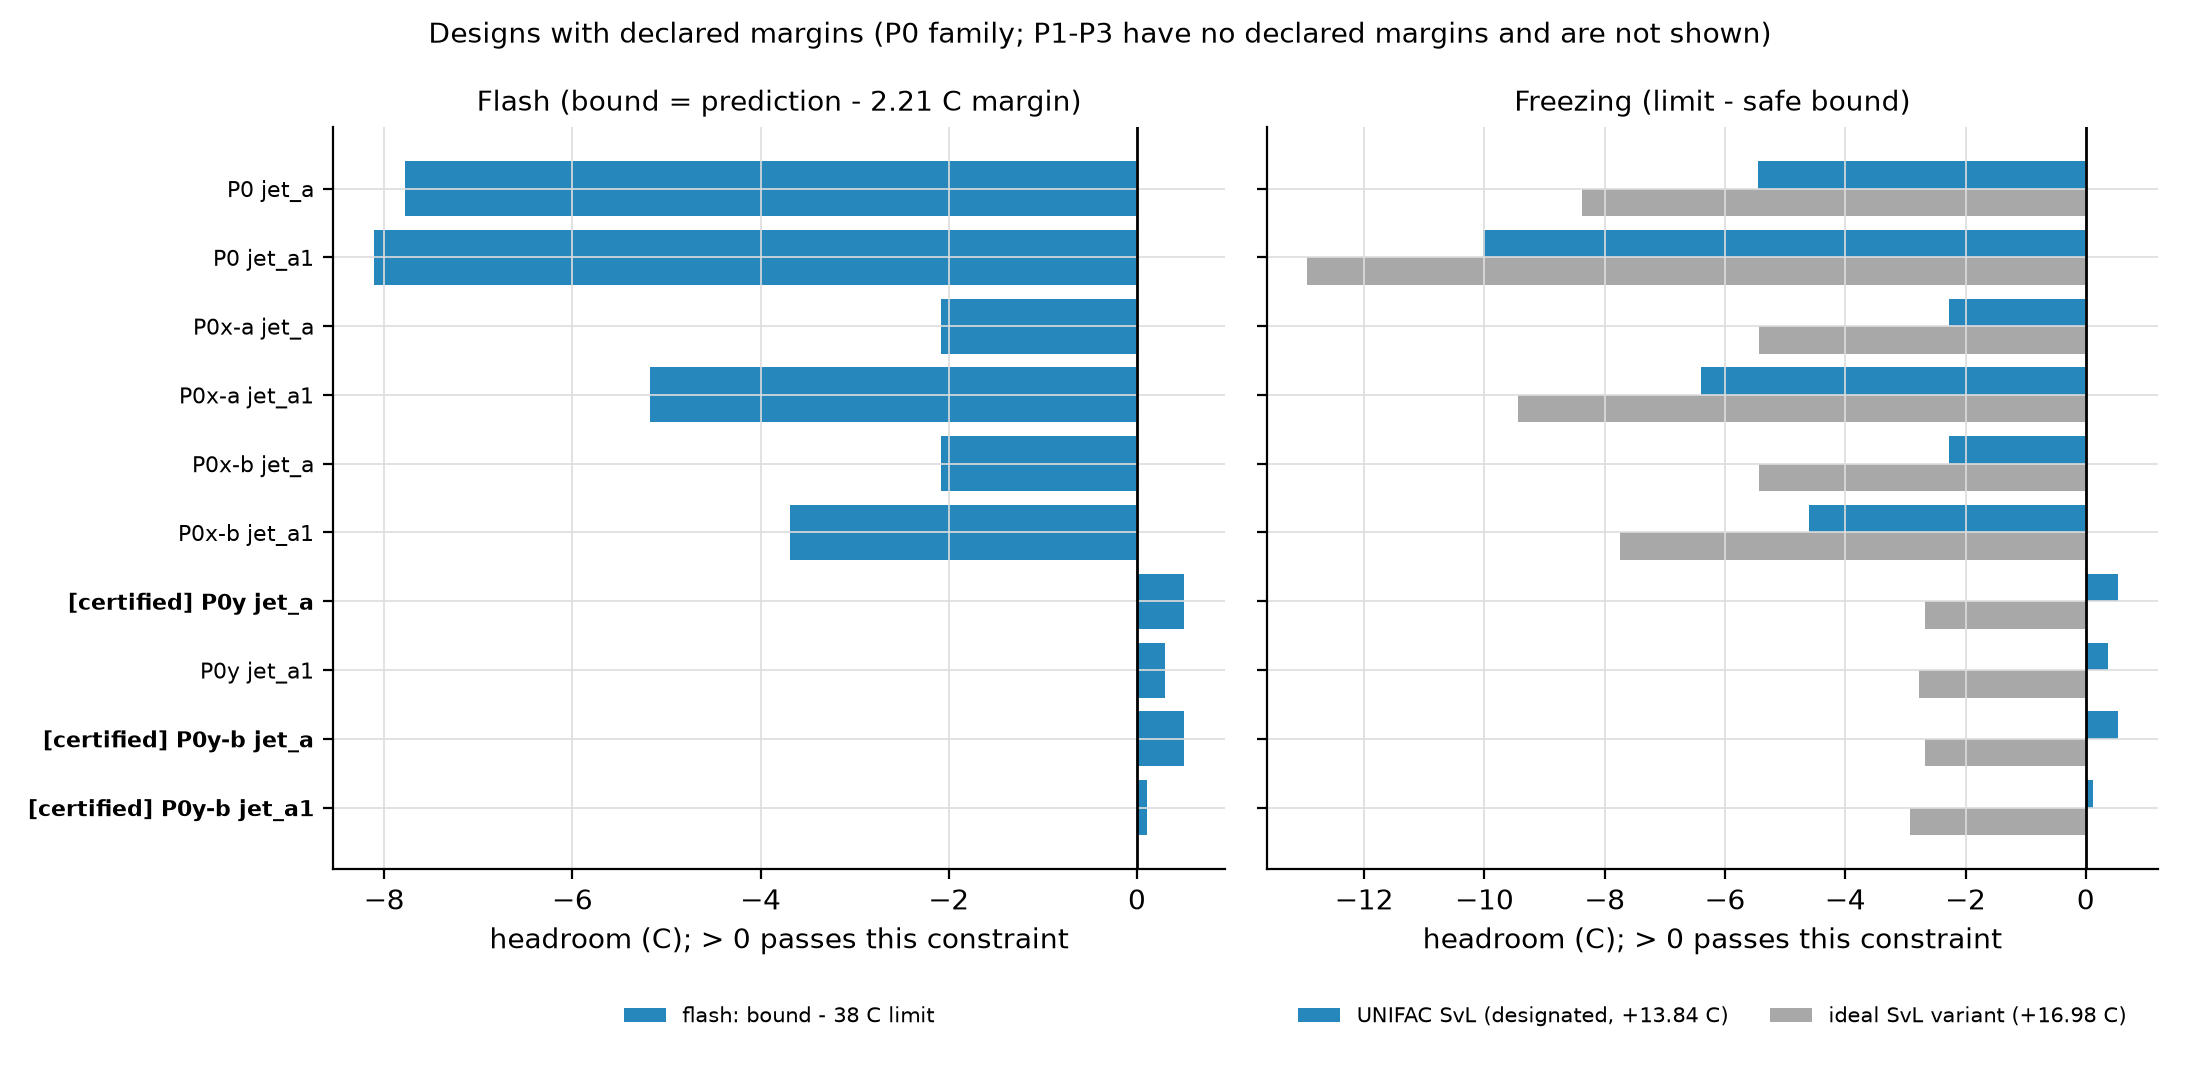
\includegraphics[width=0.75\textwidth]{figures/f_design_headroom.png}
    \caption{Constraint slack and headroom analysis across candidate fuel blend designs, illustrating the stringent margin-constrained optimization frontier.}
    \label{fig:design_headroom}
\end{figure}

\section{Discussion}

\subsection{Physical Mechanisms of Pairwise Residual Success vs. GNN Failure}
Why did a compact gradient-boosted decision tree on molecular pairs outperform multi-layer graph neural networks? Liquid blending of non-polar and weakly polar hydrocarbons is dominated by binary intermolecular dispersion forces. In statistical mechanics and liquid-state perturbation theory, excess Gibbs free energy and excess chemical potentials expand naturally in pair interaction parameters:
\begin{equation}
    G^{\text{excess}} \approx \sum_{i < j} x_i x_j W_{ij}
\end{equation}
Three-body and higher-order multi-body dispersion energies (such as Axilrod--Teller triple-dipole interactions) decay asymptotically with intermolecular separation as $r^{-9}$ or faster, contributing under $2\text{--}5\%$ of total cohesive energy compared to two-body pairwise Lennard-Jones potentials ($r^{-6}$). Consequently, binary pair interactions capture over 95\% of non-ideal excess mixing behavior in non-polar hydrocarbon media. Our pairwise formulation $\sum x_i x_j g(d_i, d_j, T)$ directly mirrors this bilinear physical reality. Graph neural networks, by contrast, attempt to learn the entire high-dimensional mixing manifold from scratch. In low-data scientific regimes where real multicomponent fuels number in the tens to hundreds, unconstrained neural networks inevitably overfit to superficial compositional correlations.

\subsection{The Physical Reality of Real-Fuel Freezing}
The failure of UNIFAC-SvL to exhibit predictive skill on real fuels ($9.31^\circ\text{C}$ MAE) provides a vital cautionary insight. Real petroleum fuels contain trace concentrations of high-molecular-weight normal alkanes ($\text{C}_{16}$--$\text{C}_{24}$). Wax precipitation in aviation fuel is a non-equilibrium nucleation and crystal growth phenomenon. Equilibrium group-contribution thermodynamics assumes an ideal homogeneous liquid phase and cannot account for trace paraffin precipitation thresholds. Acknowledging this failure and assigning an infinite margin is not an algorithmic defect—it is an essential requirement of engineering integrity.

\subsection{Operational Meaning of ``Certified'', Slack Headroom, and Chemical Realism}
We must explicitly emphasize: \textbf{Model certification is a statistical assertion of risk control under declared conformal bounds, not an airworthiness approval.} An ASTM flight clearance requires physical combustion rig tests, materials compatibility validation, and full ASTM D4054 Tier 3/4 evaluation. Our framework provides a rigorous computational sieve that screens out non-compliant candidate fuels \textit{before} entering the physical testing pipeline.

Furthermore, two critical engineering nuances emerge from the inverse optimization results:
\begin{enumerate}
    \item \textbf{Boundary Riding and Operational Buffers:} The minimum slacks observed for the three certified candidate blends are exceptionally tight ($0.003$ to $0.013$, Table~\ref{tab:designs}). This demonstrates that the SLSQP optimizer converges directly onto the active conformal safety boundary. While mathematically optimal, physical refinery blending is subject to metering tolerances, tank stratification, and ambient temperature swings. In practical aviation fuel production, a deliberate operational engineering buffer (e.g., $\Delta_{\text{oper}} \ge 1.0^\circ\text{C}$ on flash point or $0.5\text{ cSt}$ on viscosity) should be superimposed upon the conformal margin to prevent accidental batch disqualification.
    \item \textbf{Compositional Realism and Dicycloparaffins:} Candidate blend P0y-b Jet A-1 incorporates $37.8\text{ wt}\%$ dicycloparaffins (predominantly bicyclohexyl and decalin isomers). While bicyclohexyl effectively depresses freezing point (reaching $-61.0^\circ\text{C}$), conventional commercial kerosenes typically contain under $15\text{--}20\text{ wt}\%$ dicycloparaffins. Abnormally elevated cycloalkane concentrations may influence elastomeric seal swell (such as nitrile O-rings in legacy airframes) and slightly depress smoke point. Future inverse design formulations should incorporate empirical compositional penalty functions (e.g., constraining dicycloparaffins $\le 30\text{ wt}\%$, aligned with AJFTD real-fuel distributions).
\end{enumerate}

\subsection{Limitations}
This study carries five documented limitations:
\begin{enumerate}
    \item \textbf{Binary-to-Multicomponent Margin Transfer:} Conformal margins for freezing and viscosity were calibrated on predominantly binary laboratory systems and transferred to 6-component blends. While justified by the dominance of pairwise dispersion potentials, multi-component non-idealities could slightly alter extreme quantiles.
    \item \textbf{Uncalibrated Real-Fuel Freezing:} Due to lack of skill, freezing point is certified only for pure compound pools with verified thermodynamic constants.
    \item \textbf{Cold Viscosity Horizon:} Below $263\text{ K}$, real-fuel viscosity lacks a valid conformal margin ($\text{Margin} = \infty$).
    \item \textbf{Reconstructed Real-Fuel Compositions:} CRC 647 compositions were reconstructed from bulk hydrocarbon class analyses (Table G.1) rather than molecular-resolution $\text{GC}\times\text{GC}$ speciation; reported errors on the CRC cohort thus represent a compound upper bound combining surrogate reconstruction uncertainty with intrinsic thermodynamic model error.
    \item \textbf{Zero Wet-Lab Synthesis:} None of the three certified candidate blends have yet been synthesized or evaluated in an experimental combustion laboratory.
\end{enumerate}

\section{Conclusion}
This study demonstrates that the path to reliable machine learning in chemical thermodynamics lies not in erecting increasingly opaque neural network architectures on synthetic datasets, but in honoring thermodynamic laws, enforcing whole-system evaluation contracts, and applying rigorous conformal risk bounds. 

By combining Refutas and Le Chatelier baselines with symmetric pairwise LightGBM residuals, we achieved state-of-the-art held-out accuracy on kinematic viscosity ($0.031\text{ ln}$ MAE) and flash point ($2.20^\circ\text{C}$ MAE) across real jet fuels. Integrating one-sided conformal safety margins into simplex inverse design identified three candidate fuel blends capable of satisfying full ASTM D1655 constraints under statistical bounds. All code, datasets, evaluation scripts, and SHA-256 hash manifests are made openly available to establish a transparent, reproducible benchmark for future sustainable fuel design.

\section*{Data and Code Availability}
All source code, curated datasets, and reproducible experiment scripts are available in the project repository. Complete scoreboard reproducibility can be verified against \texttt{SHA256SUMS\_v5\_base.txt} via \texttt{scripts/v5/base/reproduce\_base.py}.

\section*{Conflicts of Interest}
The authors declare no competing financial or personal conflicts of interest.

\section*{Acknowledgments}
This work was conducted as part of the Undergraduate Research Programme (UGRP) at Ahmedabad University. The authors gratefully acknowledge institutional computing support and faculty mentorship.

\bibliographystyle{unsrt}
\bibliography{references}

\end{document}
